\begingroup

\TPGrid{3}{36}
\textblockorigin{0mm}{0mm}
\setlength{\parindent}{0mm}

%% bandeau identitaire
\begin{textblock*}{8.5in}(0mm,30\TPVertModule)
  \textcolor{rouge}{\rule{2\TPHorizModule}{\TPVertModule}} % bande rouge
  \textcolor{or}{\rule{\TPHorizModule}{\TPVertModule}}     % bande or
\end{textblock*}

%% logo UL
\begin{textblock*}{\TPHorizModule}(2\TPHorizModule,32\TPVertModule)
  \mbox{}
  
\includegraphics[height=2.5\TPVertModule,keepaspectratio=true]{ul_p}
\end{textblock*}

%% image de fond
\begin{textblock*}{8.5in}(0mm,0mm)
  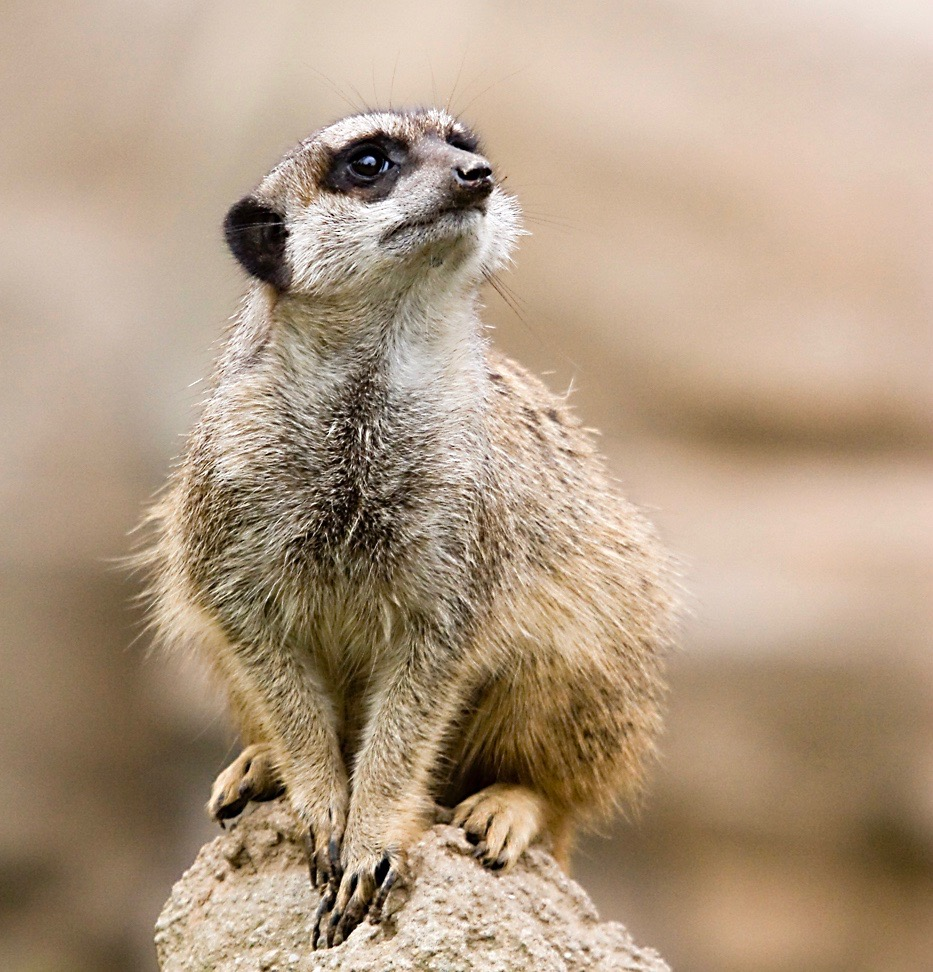
\includegraphics[height=29.95\TPVertModule,keepaspectratio=true]{Suricata.jpg}
\end{textblock*}

%% trame
\begin{textblock*}{2\TPHorizModule}(0mm,13\TPVertModule)
  \pgfsetfillopacity{0.5}
  \textcolor{white}{\rule{\linewidth}{8\TPVertModule}}
  \pgfsetfillopacity{1}
\end{textblock*}

%% titre
\begin{textblock*}{1.7\TPHorizModule}(0.3\TPHorizModule,14.2\TPVertModule)
  \thetitle
\end{textblock*}

\endgroup

%%% Local Variables:
%%% mode: latex
%%% TeX-master: "formation-latex-ul"
%%% TeX-engine: xetex
%%% End:
